%!TEX root = ../template.tex
%%%%%%%%%%%%%%%%%%%%%%%%%%%%%%%%%%%%%%%%%%%%%%%%%%%%%%%%%%%%%%%%%%%%
%% chapter2.tex
%% NOVA thesis document file
%%
%% Chapter with the template manual
%%%%%%%%%%%%%%%%%%%%%%%%%%%%%%%%%%%%%%%%%%%%%%%%%%%%%%%%%%%%%%%%%%%%

%%-------------------------------------------------------------------
%%	2 - Related Work
%%-------------------------------------------------------------------
\chapter{Related Work}
\label{cha:related_work}

The focal point of this dissertation is the challenges of implementing a distributed system based on a file system, that can store \textit{VMs} images and leverage the benefits of snapshot and caching techniques. Moreover, it is intended that the proposed solution integrates smoothly into a broader infrastructure.

This chapter will address the central concepts and associated technologies encompassed in this work, particularly: \\
\begin{description}
	\item [Section~\ref{sec:virtualization}] overviews virtualization as a core concept and discuss in particular the data and metadata storage method.
	%
	\item [Section~\ref{sec:storage}] studies the principal characteristics of a file system, with emphasis on snapshot techniques and replication and consistency models.

\end{description}

%%-------------------------------------------------------------------
%%	2.1 - Virtualization
%%-------------------------------------------------------------------
\section{Virtualization} % (fold)
\label{sec:virtualization}

Most of today's machines have such a level of performance that allows the simultaneous execution of multiple applications and the sharing of these resources by several users. In this sense, it is natural to have a line of thought in which all available resources are efficiently used. 

Virtualization is a technique that allows for the abstraction of the hardware layer and provides the ability to run multiple workloads on a shared set of resources. Nowadays, virtualization is an integral part of many \textit{IT} sectors with applications ranging from hardware-level virtualization, operating system-level
virtualization, and high-level language virtual machines.
\nocite{VMware_VM2006}



A virtual machine (VM) by design is an efficient, isolated duplicate of a real machine~\cite{Popek1974}, in that order, it was the capacity to virtualize all of the hardware resources, including processors, memory, storage, and network connectivity.

To manage the VMs, there is a need for a layer of software that has certain characteristics. One of them is the capability to provide an environment in which VMs conduct operations, acting both as a controller and a translator between the VM and the hardware for all \textit{IO} operations. This is known as a virtual machine monitor (VMM), or more common at this moment a \textit{hypervisor}.


% section virtualization (end)


%%-------------------------------------------------------------------
%%	2.1.X - Hypervisors
%%-------------------------------------------------------------------
\subsection{Hypervisors} % (fold)
\label{sub:hypervisors}

The most important aspect of running a VM is that it must provide the illusion of being a real machine, allowing to boot and install any operating system (OS). It is the hypervisor which has that task and should do it in an efficient manner at the same time providing this three properties~\cite{Popek1974}:

\begin{description}
	\item[Fidelity:] a program should behave on a VM the same way or in much the same way as if it were running on a physical machine.
	%
	\item[Performance:] much of the instructions in the virtual machine should be executed directly by the real processor without intervention by the hypervisor.
	%
	\item[Isolation:] the hypervisor must have complete control over the resources. 
\end{description}

An hypervisor can be classified into two different types, symbolising two different design strategies to virtualization, as shown in Figure~\ref{fig:hypervisors}:

%\begin{figure}[htbp]
%	\centering
%	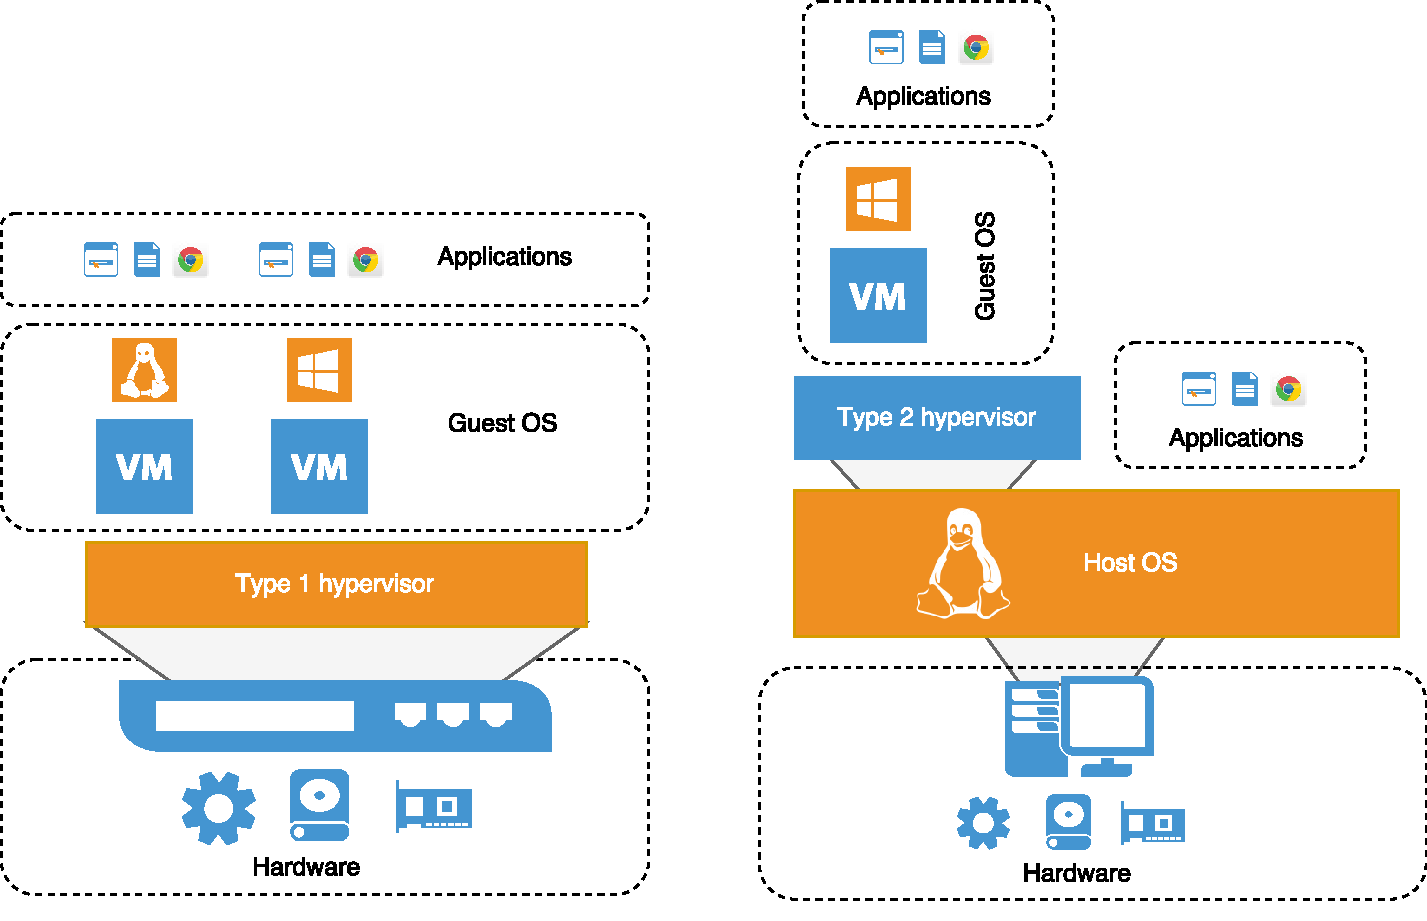
\includegraphics[height=4in]{cap2_hypervisorsv2}
%	\caption{Virtualization architecture with type 1 and type 2 hypervisors}
%	\label{fig:hypervisors}
%\end{figure}

\begin{description}
	\item [Type 1 hypervisor:] sometimes referred as a bare-metal hypervisor, are very similar to an operating system since they run directly on the hardware and are the only program executed by the CPU in the most privileged mode. As there isn't a go-between itself and the resources, being able to communicate directly to the hardware, this type of hypervisor presents as a more efficient solution than the type 2 hypervisor.
	%
	\item [Type 2 hypervisor:] In comparison, this kind of hypervisor relies on an already installed operating system, and acts very similarly as any conventional process. Having the need to request resources to the OS underneath. On the other hand, there are some advantages. Mainly this solution is easier to deploy since the work of supporting the hardware is already done by the OS below.
\end{description}

Either way, the challenge lays in the fact that the hypervisor needs to execute the guests OS instructions in a safe manner and at the same time provide possible different machine configurations to each of them. These characteristics, such as the number and architecture of virtual CPUs (vCPU), the amount and type of memory available (vRAM), the allowed space to store files (vDisk), and so on, are user configurable but is the hypervisor that is tasked to do the management and load balancing. The settings of all these components are compiled in a VM configuration file. In the case of VMware hypervisors, the file employs the \texttt{.vmx} extension.\cite{VMWare_VMFiles,Portnoy2012}

With a virtualized infrastructure there is an opening for a substantial reduction in the number of servers. Which in turn diminishes the setup time of a server as those VMs are commonly created with a resource to cloning techniques. Software updates can be greatly simplified and made available to all users at once. Even availability is improved since it is an easy task to launch a new VM from a template and migrate all the services that were being made reachable by one that suffered a failure. 

% subsection hypervisors (end)



%%-------------------------------------------------------------------
%%	2.1.X - VDI
%%-------------------------------------------------------------------
\subsection{Virtual Desktop Infrastructure} % (fold)
\label{sub:vdi}

%\begin{figure}[htbp]
%	\centering
%	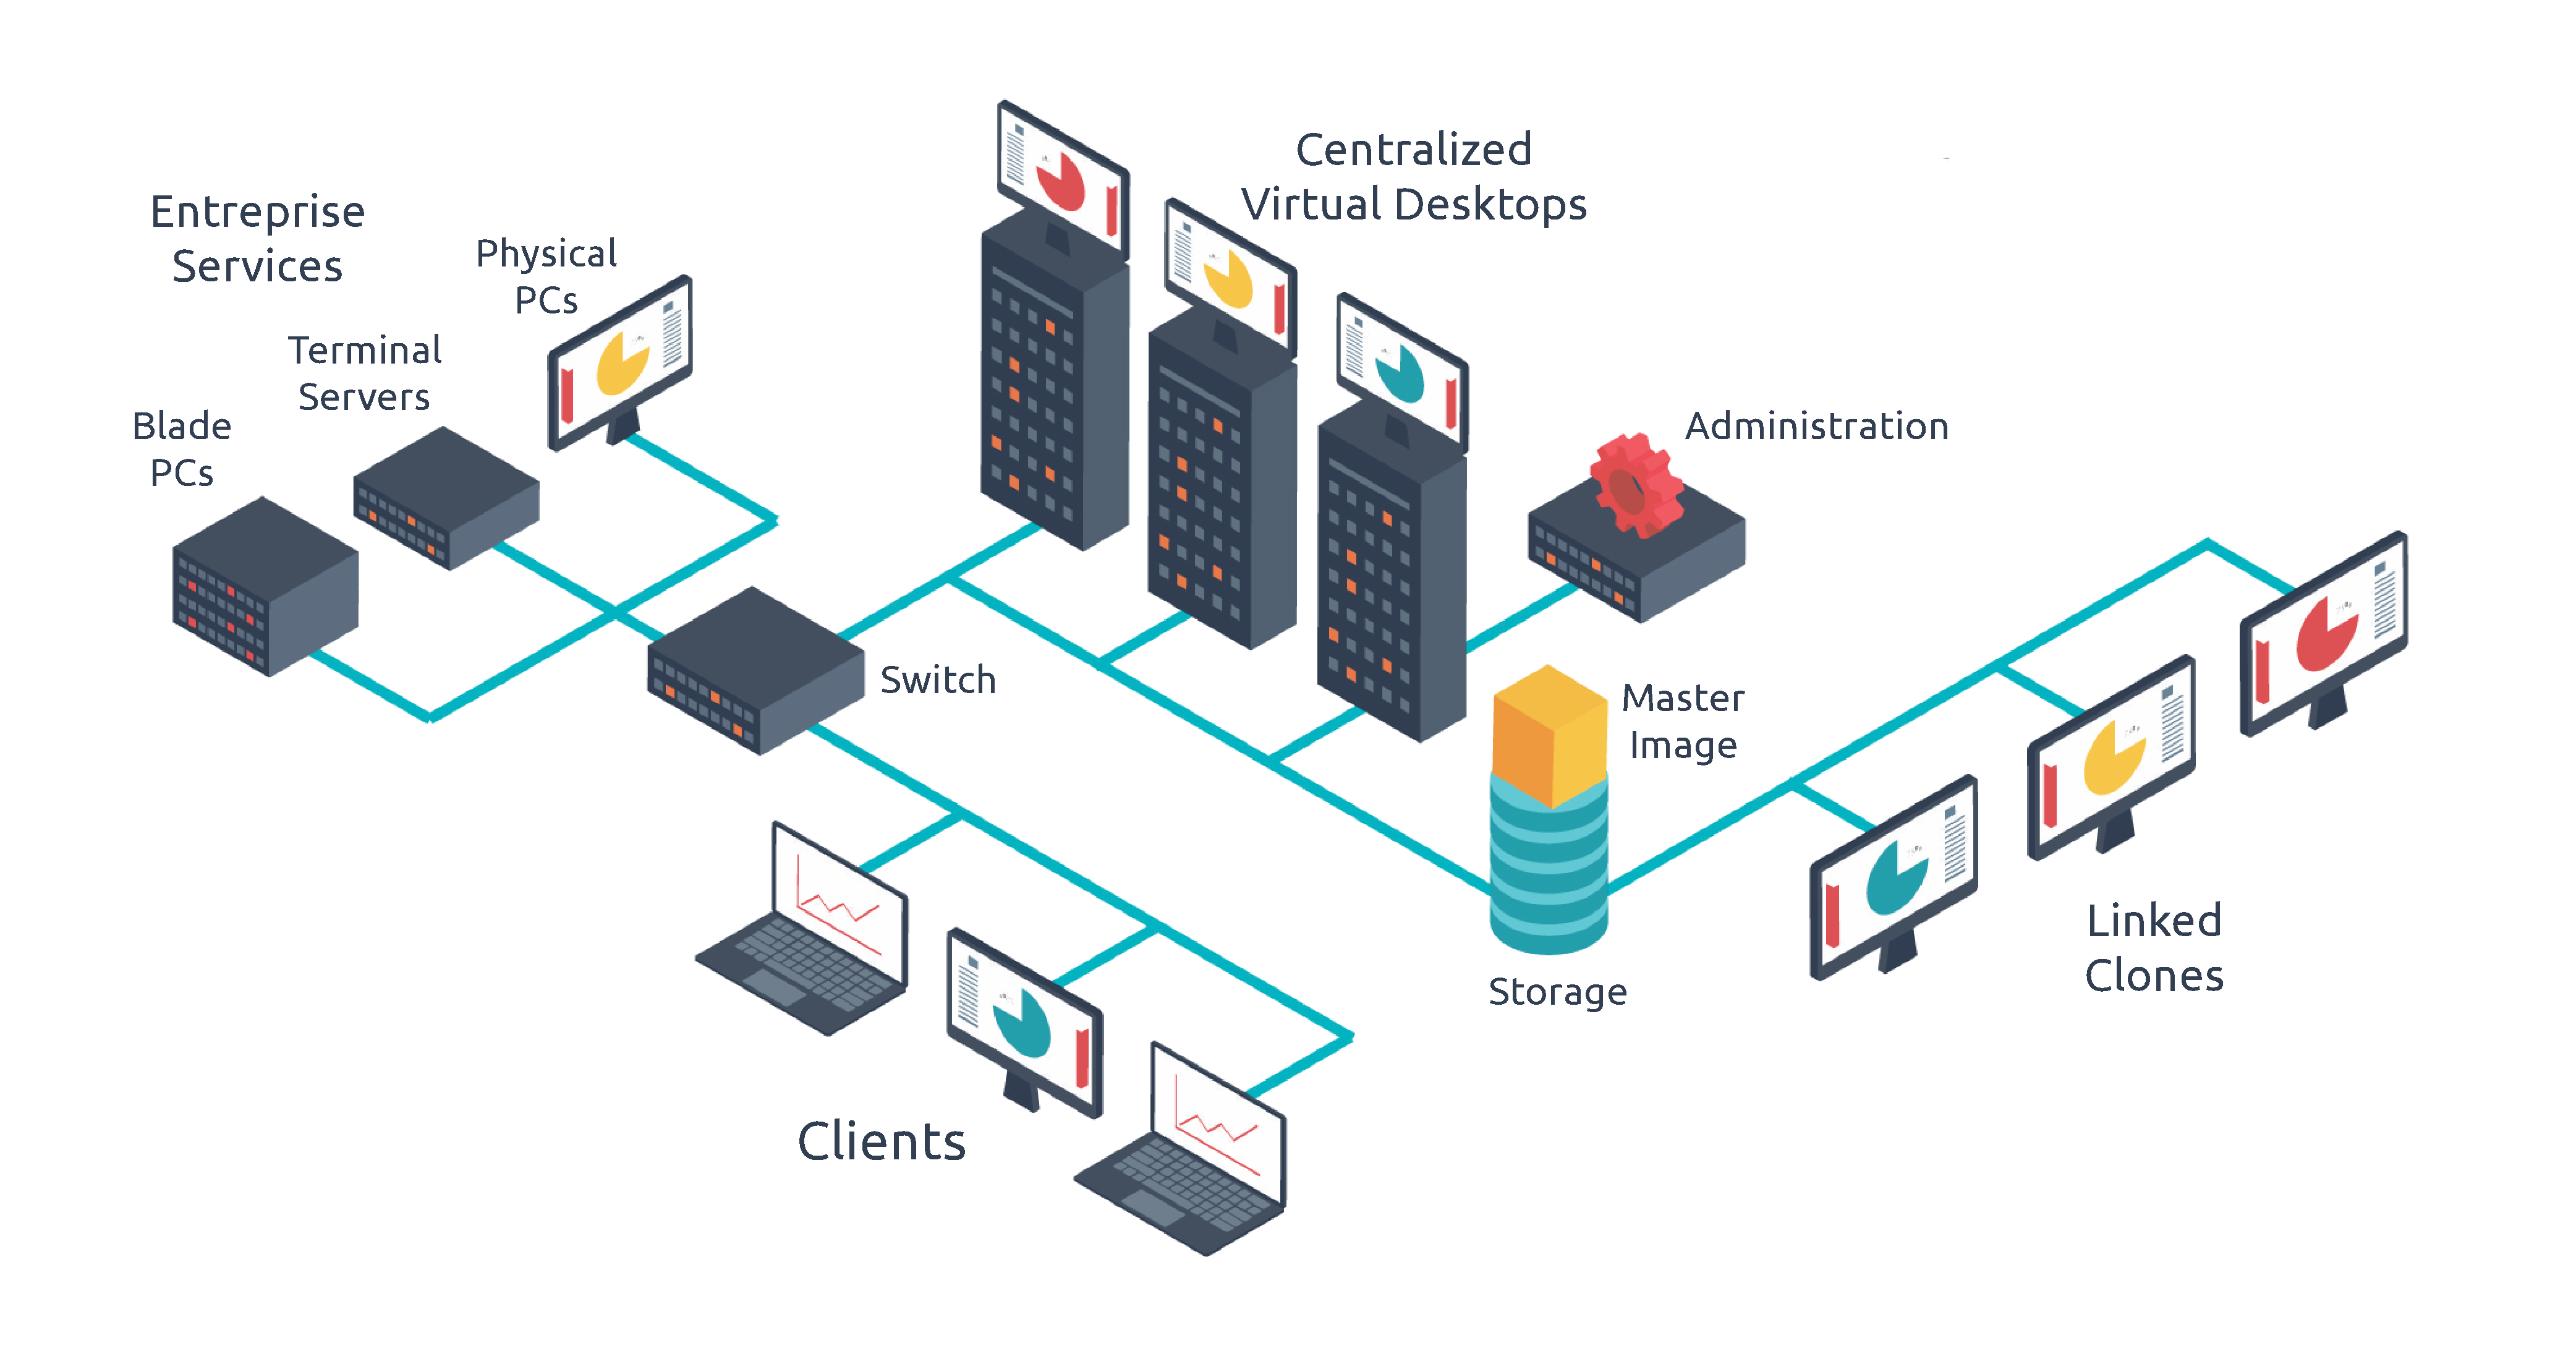
\includegraphics[height=3in]{cap2_VDIv2}
%	\caption{An exemple of a Virtual Desktop Infrastructure, adapted from AppDS~\cite{appds_2017}}
%	\label{fig:VDI}
%\end{figure}

It is common to find in a typical midsize corporate infrastructure hundreds of servers and thousands of workstations. All in a diverse ecosystem counting with many hardware configurations, different OSs and applications needs. Probably even supporting several versions of the same software required for the day to day operations.

One solution to the predicament above is to use virtualization as a mechanism for virtualizing the complete workstation. The implementation with more relevance and with more expression at the moment is the virtual desktop infrastructure (VDI).

The concept encompasses a series of techniques, providing on demand availability of desktops, in which, all computing is performed employing virtual machines~\cite{VMWare_VDI2006}.
Typically this solution presents a centralised architecture, where the user's environment resides on a server in a data centre, as shown on Figure~\ref{fig:VDI}. However, other components are required, such as storage for the users and VMs data and a network capable of moving large data blocks quickly, all in a perspective where from the user's viewpoint there can't be any apparent difference between a virtual desktop and a local installation.

There are two antagonistic approaches to the architecture, one focused on the server-side and the other on the client-side:

\begin{description}
	\item [Server-based VDI] This is the most common approach, in which the VM runs remotely on a server using a hypervisor. Featuring such benefit, as the fact that only a low-performance thin client with support for a protocol such as Remote Desktop Protocol (RDP)~\cite{Microsoft_RDP} or the Remote Framebuffer Protocol (RFB)~\cite{rfc6143} is required to interact with the virtual desktop.

		The downside involves the costs necessary to maintain the service. A powerful support infrastructure is needed (computing, storage, networking and power). With a need in some use cases to add high-end graphics processors to satisfy the workflow of customers using multimedia tools. Moreover, the computational strength of the hardware present in the clients is not harnessed. 

		There are plenty of commercial solutions that use this principle, with the three largest players being VMware's Horizon platform~\cite{VMware_horizon}, XenDesktop from Citrix~\cite{Citrix_XenDesktop} and Microsoft with Microsoft Remote Desktop~\cite{Microsoft_RDS}.
	%
	\newpage
	\item [Client-based VDI] There is another case, where the VM is executed directly on the client machine. Here the local hardware is fully handled by one hypervisor, giving some slack to the infrastructure servers that just need to perform management and storage tasks on the platform.

		Although this approach presents itself as significantly more cost restrained, there isn't a notable adoption by software houses in developing products in this family. One of the possible reasons may be that previously existing solutions, such as Citrix's XenClient~\cite{Citrix_XenDesktop}, needed to erase the user machine disk completely~\cite{VMblog_Citrix}.
\end{description}

As discussed earlier virtualization has paved the way for a class of services called IaaS. That leads to an apanage of modern times in which there is a desire to link all services to the cloud; so it is natural that an idea came to take the VDI paradigm to this medium. Thus giving rise to the emergence of Desktop as a Service (DaaS), with companies such as Amazon, VMware and Citrix entering the market.

This model has a real potential for cost minimization since there is no need for concern in regards to the maintenance and acquisition of the infrastructure. Since the organisation only has to make available the workstations and a way of establishing a connection to the service. Although, there is always a dependence on the network conditions such as large latencies and low bandwidth.

\nocite{Nuno2016}
\nocite{Eduardo2016}
\nocite{P2020}

% subsection vdi (end)


%%-------------------------------------------------------------------
%%	2.1.X - VM storage
%%-------------------------------------------------------------------
\subsection{Virtual Machine Image Storage} % (fold)
\label{sub:vm_storage}

The data storage is the focal point to address in this work. Therefore, it is important to understand how a virtual machine is composed and how is translated to a representation in a storage device.

The representation of a machine's settings and state more the information about snapshots comprise to a set of metadata. On the other hand, the Operating System, applications, logs and snapshots constitute the remaining data. Such data and metadata must be saved in a storage system, regardless of type, but is typically defined by a set of files. 

Given the architecture presented by VMware software~\cite{VMWare_VMFiles}, the main files required for the operation of a VM are:

\begin{itemize}
	\item The VM configuration file - The \texttt{.vmx} file holds the fundamental configuration options, describing every aspect of the VM.
	%
	\item The virtual disk files - Embodying multiple \texttt{.vmdk}, which stores the contents of the virtual machine's hard disk drive.
	%
	\item The file that stores the BIOS - The \texttt{.nvram} file stores the state of the virtual machine's BIOS.
	%
	\item The suspended state file - The \texttt{.vmss} saves contains the state of a suspended virtual machine.
	%
	\item Log files - A collection of \texttt{.log} files is created to log information about the virtual machine and often handled for troubleshooting purposes.
\end{itemize}


In addition to the records described above, there may be some more related to the use of snapshots. The implementation of snapshots can be described as follows: first, the state of the resource is stored in the form of an immutable and persistent object, and second all modifications that transform the state of the resource are saved in a different object. To save this objects the \texttt{.vmsn} extension is employed.
The snapshotting technique is discussed in a more comprehensive sense in the Section~\ref{sub:snapshots}.

% subsection vm_storage (end)


%%-------------------------------------------------------------------
%%	2.2 - Storage
%%-------------------------------------------------------------------
\section{Storage} % (fold)
\label{sec:storage}

As stated in previous sections, the main problem to be addressed in this work is the storage concerning virtual machines. That could be either images, snapshots, files or data structures that are needed to support the execution of a VM. 

When applied to the VDI concept some demands appear in the form of a specific care at planning the storage system architecture, as well as the supporting infrastructure: the hardware picked, network topology, protocols used, and software implemented.

At the end of the day, the idea is to present a solution that offers an appropriate cost to performance ratio, and that with little effort can scale when the need emerges.


% section storage (end)


%%-------------------------------------------------------------------
%%	2.2. - File Systems
%%-------------------------------------------------------------------
\subsection{File Systems} % (fold)
\label{sub:file_systems}

The traditional and perhaps most common way of storing files and, in turn, VMs is the use of file systems.
This kind of system is used to manage the way information is stored and accessed on storage devices. A file system can be divided into three broad layers, from a top-down perspective we havew:

\begin{itemize}
	\item The \textbf{Application Layer} is responsible for mediating the interaction with user's applications, providing an API for file operations. This layer gives file and directory access matching external names adopted by the user to the internal identifiers of the files. Also, manages the metadata necessary to identify each file in the appropriate organisational format.
	%
	\item Then the \textbf{Logic Layer} is engaged in creating a hardware abstraction through the creation of logical volumes resulting from the use of partitions, RAID volumes, LUNs, among others.
	%
	\item The last one is the \textbf{Physical Layer}. This layer is in charge with the physical operations of the storage device, typically a disk. Handling the placement of blocks in specific locations, buffering and memory management.
\end{itemize}


There are many different types of file systems, each one boasting unique features, which can range from security aspects, a regard for scalability or even the structure followed to manage storage space.

\begin{description}
	\item [Local file systems:] A local filesystem can establish and destroy directories, files can be written and read, both can move from place to place in the hierarchy but everything contained within a single computing node. 
Good performance can be improved in certain ways, incorporating caching techniques, read ahead, and carefully placing the blocks of the same file close to each other, although scalability will always be reduced. 
There are too many file systems of this genre to be here listed. Nevertheless, some of the most renowned may be mentioned. As the industry-standard File Allocation Table (FAT), the New Technology File System (NTFS) from Microsoft, the Apple's Hierarchical File System Plus (HFS+) also called Mac OS Extended and the B-tree file system (BTRFS) initially designed by Oracle.
	% 
	\item [Distributed file system:] A distributed file system enables access to remote files using the same interfaces and semantics as local files, allowing users to access files from any computer on a network. 
	Distributed file systems are being massively employed in today's model of computing. They offer state-of-the-art implementations that are highly scalable, provide great performance across all kinds of network topologies and recover from failures. 
	Because these file systems carry a level of complexity considerably higher than a local file system, there is a need to define various requirements such being transparent in many forms (access, location, mobility, performance, scaling). As well as, handle file replication, offer consistency and provide some sort of access-control mechanisms. 
	All of these requirements are declared and discussed in more detail in the book \enquote{Distributed Systems: Concepts and Design} by George Coulouris et al.~\cite{Coulouris2011}
	We can give as example of file systems the well-known Network File System (NFS)~\cite{rfc5661} originally developed by Sun Microsystems, and the notable Andrew File System (AFS)~\cite{Satyanarayanan1990} developed at Carnegie Mellon University.
\end{description}


In this work, the snapshot functionality of the file system itself is a valuable asset. This technique is present in some of the most recently designed file systems, such as the BTRFS. It has already been mentioned that previous work has been done to use the file system snapshot features as a base feature. This way the creation of linked-clones handled by the file system capabilities as an alternative to linked-clones created by virtualization software itself.


There are numerous types of additional file systems not mentioned since they are not in the domain of this work. Still, it is important to note the existence of an architecture that is not similar to the traditional file hierarchy adopted in file systems, which is the object-based storage. 

This structure, as opposed to the ones presented above, manages data into evenly sized blocks within sectors of the physical disk. It is possible to verify that it has gained traction leading to the advent of the concept of cloud storage. There are numerous implementations of this architecture, whether in small local deployments or large-scale data centres supporting hundreds of petabytes of data.
This type of file system is being studied in the context of a parallel thesis but inserted in the same project already presented.

It is worthwhile to enumerate some examples such as CephFS~\cite{Weil2006}, OpenStack Swift~\cite{Swift2017}, and in a IaaS flavour the Amazon S3~\cite{aws_s3} and Google Cloud Storage~\cite{gcp_storage}.

% section file_systems (end)


%%-------------------------------------------------------------------
%%	2.2. - Snapshots
%%-------------------------------------------------------------------
%\subsection{Snapshots} % (fold)
%\label{sub:snapshots}

%\textbf{TO DO - Expand}

%In this work, we propose to use the snapshot functionality of the file system itself, present in some of the most recently designed file systems, such as the BTRFS. This way the creation of linked-clones handled by the file system capabilities as an alternative to linked-clones created by virtualization software itself.


% section snapshots (end)


%%-------------------------------------------------------------------
%%	2.2. - Caching
%%-------------------------------------------------------------------
\subsection{Caching} % (fold)
\label{sub:caching}

A cache can be defined as a store of recently used data objects that is nearby one client or a particular set of clients than the objects themselves. The inner works of one of these systems are rather simple. When a new object is obtained from a server, it is added to the local cache, replacing some existing objects if needed. That way when an object is requested by a client, the caching service first checks the cache and supplies the object from there if an up-to-date copy is available. If not, an up-to-date copy is fetched, then served to the client and stored in the cache. 

Caching often plays a crucial role in the performance and scalability of a file system and is used extensively in practice.

Caches may be found beside each client or they may be located on a server that can be shared by numerous clients.

\begin{description}
	\item [Server-side Cache:] Server side caching is when the caching data occur on the server. There is no right way to the approach of caching data; it can be cached anywhere and at any point on the server assuming it makes sense. It is common to cache frequently used data from a DataBase to prevent connecting to the DB every time some data is requested. In a web context, it is common to cache entire pages or page fragments so that there is no need to generate a web page every single time a visitor arrives.
	%
	\item [Client-side Cache:] Maintaining the analogy to the Web environment, caches are also used on the client side. For instances, Web browsers keep a cache of lately visited web pages and other web resources in the client’s local file system. Then when the time comes to serve a page that is stored in the cache, a special HTTP request is used to check, with the corresponding server, if the cached page is up-to-date. In a positive response the page is simply displayed from the cache, if not, the client just needs to make a normal request.
\end{description}

\newpage
% section caching (end)


%%-------------------------------------------------------------------
%%	2.2. - Replication and Consistency
%%-------------------------------------------------------------------
\subsection{Replication} % (fold)
\label{sub:replication_consistency}

At the storage level, replication is focused on a block of binary data. Replication may be done either on block devices or at the file-system level. In both cases, replication is dealing with unstructured binary data. The variety of technologies for storage-level replication is very extensive, from commodity RAID arrays to network file system.
File-based replication works at a logical level of the storage system rather than replicating at the storage block level. There are multiple different methods of performing this. And, unlike with storage-level replication, these solutions almost exclusively rely on software.

Replication is a key technology for providing high availability and fault tolerance in distributed systems. Nowadays, high availability is of increasing interest with the current tendency towards mobile computing and consequently the appearance of disconnected operation. Fault tolerance is an enduring concern for does who provide services in critical and other important systems.

There are several arguments for which replication techniques are widely adopted; these three are of significant importance:

\begin{description}
	\item [Performance improvement:] Performance improvement: Replication of immutable data is a trivial subject, is nothing more than a copy of data from one place to another. This increases performance, sharing the workload with more machines with little cost within the infrastructure.
	%
	\item [Increased availability:] Replication presents itself as a technique for automatically keeping the availability of data despite server failures. If data is replicated in additional servers, then clients may be able to access that data from the servers that didn't experience a failure.
Another factors that must be taken into account are network partitions and disconnected operation.
	%
	\item [Fault tolerance:] There is the need o maintain the correctness guarantees of the data in the appearance of failures, which may occur at any time.
\end{description}

%CAP theorem states that it is impossible for a distributed computer system to simultaneously provide all three of the following: Consistency , Availability and Partition tolerance .

%Consistency (all nodes see the same data at the same time)
%Availability (every request receives a response about whether it succeeded or not)
%Partition tolerance (the system continues to operate despite arbitrary message loss or partial failure of the system or unavailability due to network partitions)

% section replication_consistency (end)




 
